\documentclass[10pt]{article}
\usepackage{amsmath}
\usepackage{amssymb}
\usepackage{graphicx}
\usepackage{cite}
\usepackage{color} 

\topmargin 0.0cm
\oddsidemargin 0.5cm
\evensidemargin 0.5cm
\textwidth 16cm 
\textheight 21cm

% Bold the 'Figure #' in the caption and separate it with a period
% Captions will be left justified
\usepackage[labelfont=bf,labelsep=period,justification=raggedright]{caption}

% Use the PLoS provided bibtex style
\bibliographystyle{plos2009}

% Remove brackets from numbering in List of References
\makeatletter
\renewcommand{\@biblabel}[1]{\quad#1.}
\makeatother


% Leave date blank
\date{05/16/2014}

\pagestyle{myheadings}

\begin{document}

% Title must be 150 characters or less
\begin{flushleft}
{\Large
\textbf{Galaxy Zoo: Identifying galaxies}
}
% Insert Author names, affiliations and corresponding author email.
\\
Jeffrey Ning, 
Darshan Hegde 
\\
jkn233@nyu.edu, dh1806@nyu.edu
\end{flushleft}

\section*{Introduction}


\section*{Problem Definition}

\section*{Methodology}

\section*{Feature Description}

\subsection*{Histogram of Gradients (HoG) Features}
We first convert the image to grayscale. We crop the center $ 208 \times 208 $ pixels and resize it down to $104 \times 104$. We then calculate HoG features as follows. Given an image, we first take a small $k \times k$ patch of image ($8 \times 8$ pixels in our case), and we calculate gradient vectors for each pixel. Then we build a histogram with r bins ( 8 bins in our case), each bin corresponds to ${[(180/r)i, (180/r)(i+1)]} , i=\{0, .. (r-1)\}$. Each bin contains sum of magnitudes of all gradient vectors in that bin. We do this for all patches in the image and concatenate all the histogram vectors. We only consider non overlapping patches, so for $104 \times 104$ image, we have 169 patches by $8 \times 8$ patch size. Our HoG features have dimension of 1352. The image below shows the HoG calculations on a sample image: 

\begin{center}
\begin{figure}[h]
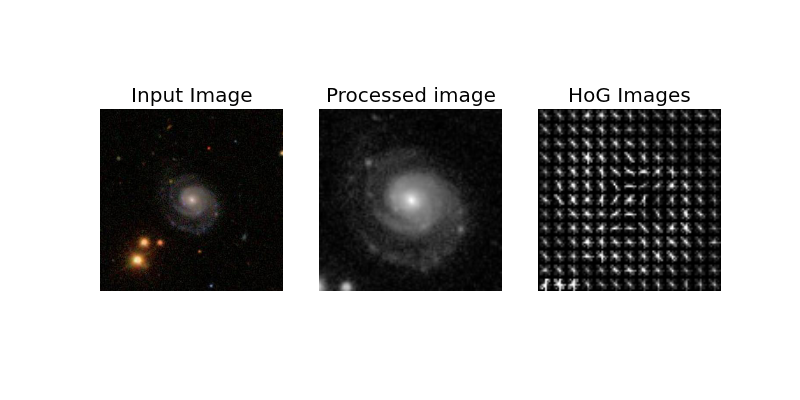
\includegraphics[scale=0.8]{images/HoG_features_noisy.png}
\caption{HoG Feature Transformation}
\label{fig:hog}
\end{figure}
\end{center}


\subsection*{Raw Pixel based Features}

\section*{Model Description}

\subsection*{Decision Tree Regression}
Decision tree regression is a very simple non-linear regression technique. Using training data, we obtain tree structure, which is basically the series of questions about features. Inference involves, running an image through series of yes / questions (In our case, questions corresponds to a pixel and a threshold value for the pixel [Eg: $pixel(22, 23) >= 54$]). After reaching the corresponding leaf in the tree, the probability values for all 3 classes are averaged to get the prediction for that image.   

The training objective is to get leaf nodes such that, training examples which end up in the same leaf node have very close target values. Closeness of target values are measured by mean square error. Mean square error over the entire training set is defined as:

$$MSE = {1 \over n}  \sum_{c \in leaves(T)} \sum_{i \in c} (y_i - m_c)^2$$

where, $m_c =  {1 \over n_c} \sum_{i \in c} y_ic$. $m_c$ is the prediction for that leaf c. We can't do a direct minimization, so we a greedy search. We start by finding the one binary question which minimizes the MSE; this gives us our root node and two child nodes. At each child node, we repeat our initial procedure, asking which question would give us the minimum MSE, given where we already are in the tree. We repeat this recursively. There are several criteria to decide when to stop the recursion. We can set a maximum depth for the tree or minimum samples per leaf or minimum samples a leaf need to have to be considered for splitting. We choose to the last criterion and decide the threshold using cross-validation.

The basic regression-tree-growing algorithm then is as follows:

\begin{itemize}
  \item Start with a single node containing all points. Calculate $m_c$ and MSE.
  \item Search over all binary splits ( pixel and threshold for the pixel ), and find the split that results in minimum MSE, and use the split to create child nodes.
  \item In each child node, consider the node if number of examples are above the threshold. Else, stop splitting that node and consider next child, re-curse \ldots
\end{itemize}

\subsection*{Random Forest Regression} 

Random forest regression, is an ensemble method which fits $n$ number of decision trees and averages their results. While building decision trees, it uses MSE to measure the quality of split and considers only a random subset of $ \log_2(total features)$, to do each split. By considering random subset of features during each split, each decision tree in random forest look very different from each other, which is very desirable. Because, they fit different parts of feature space well.  

\subsection*{Lasso Regression}

Lasso is $L_1$ regularized linear regression. The cost function used is:

$${1 \over (2*n_samp)} \| y -Xw \|^2 + \alpha * \| w \|_1$$

Where y is target $(n\_samp \times 3)$, $X (n\_samp \times n\_feat)$ is input feature matrix and w $(n\_feat \times 3)$ is parameter matrix. The scikits-learn implementation uses coordinate descent to optimize the above cost function. Since lasso uses L1 penalty, one interesting property is that, it tries to find as sparse weight vectors are possible. In our case, since we expect only few pixels to be informative, we use this model. The model is linear, it is not well suitable for vision tasks using very low level features such as HoG, raw pixels. But, it's a good baseline model to compare the results and for doing sanity check of the coding framework, because it's relatively fast to run.

\section*{Discussion}


\section*{Acknowledgments}

\bibliography{template}


\end{document}

